\documentclass[11pt, a4paper]{article}
\usepackage[utf8]{inputenc}
\usepackage{fullpage}
\usepackage{graphicx}
\usepackage{markdown}
\usepackage{mathtools}
\usepackage{wrapfig}
\usepackage{tabu}
\usepackage{colortbl}
\usepackage[hidelinks]{hyperref,xcolor}
\usepackage[backend=biber]{biblatex}
\usepackage{adjustbox}
\usepackage{nomencl}
\renewcommand\UrlFont{\color{blue}\rmfamily}
\addbibresource{projectplan.bib}
\addbibresource{prr.bib}

\title{Preliminary Research Report\\Remote Water Sensing using UAVs}
\author{Robin \textsc{Westerik}}
\newcommand{\supervisors}{Jan \textsc{Bollen}\\Harry \textsc{Futselaar}}

\newcommand{\timePeriod}{February 2022 - June 2022}
\newcommand{\sprint}{Analyze}
\newcommand{\homepage}{\url{https://github.com/organizations/remotewatersensing/}}
\date{\today}

\makeatletter{}

\makenomenclature
\renewcommand{\nomname}{}

\begin{document}

\input{./title.tex}
\nomenclature{\(UAV\)}{Unmanned Aerial Vehicle}
\nomenclature{\(BOM\)}{Bill of Materials}
\nomenclature{\(PDR\)}{People's Democratic Republic}
\nomenclature{\(InSAR\)}{Interferometric synthetic-aperture radar}
\nomenclature{\(ENSO\)}{El Niño-Southern Oscillation}
\nomenclature{\(Indymo\)}{Innovative Dynamic Monitoring}
\nomenclature{\(ROV\)}{Remotely Operated Vehicle}
\nomenclature{\(3D\)}{Three-Dimensional}
\nomenclature{\(MAVLab\)}{Micro Air Vehicle Lab}
\nomenclature{\(IADC\)}{International Association of Dredging Companies}
\nomenclature{\(ppm\)}{Parts per million}
\nomenclature{\(FSR\)}{Full Scale Range}
\nomenclature{\(NTU\)}{Nephelometric Turbidity Unit}
\nomenclature{\(JTU\)}{Jackson Turbidity Unit}
\nomenclature{\(ORP\)}{Oxidation-Reduction Potential}
\nomenclature{\(TDS\)}{Total Dissolved Solids}
\nomenclature{\(DIY\)}{Do It Yourself}
\nomenclature{\(GPS\)}{Global Positioning Unit}
\nomenclature{\(SDK\)}{Software Development Kit}
\nomenclature{\(IP\)}{Ingress Protection}
\nomenclature{\(ESC\)}{Electronic Speed Controller}
\nomenclature{\(GPIO\)}{General Purpose Input Output}
\nomenclature{\(fps\)}{Frames per second}
\nomenclature{\(PET\)}{Polyethylene terephthalate}
\nomenclature{\(CAD\)}{Computer-Aided Design}
\nomenclature{\(DO\)}{Dissolved Oxygen}

\tableofcontents
\pagebreak

\section{Abbreviations}
\sffamily\footnotesize
\printnomenclature
\rmfamily\normalsize

\section{Introduction}

In this report, existing water sensoring solutions, quality standards, the Mekong Delta and suitable drones will be analyzed. Literature will be reviewed, and findings of which will be contained in a related studies section as well as referenced throughout the document. This document can be extended during other sprints, when new info related to the project is found. A change log as well as the git version control system \cite{git} will keep track whenever this document is edited. 

\newpage
\section{Mekong Delta}

In order to know what variables need to be monitored in the Mekong Delta, it is important to define the problems that it faces. In this section, these problems will be illustrated using various sources. This section will conclude with a definition of parameters which are most important to measure.\\

The Mekong River is one of the last large rivers on Earth not dammed for most of its length, flowing freely to the sea through five countries: Myanmar, Lao PDR, Thailand, Cambodia and Vietnam.  It discharges 16,000 cubic meters of water per second. The Mekong Basin is home to about 65 million people, of which 80\% live in the lower basin. The river is also rich in diversity, hosting about 800 fish species and over 20,000 plants. \cite{worldatlas}

The Mekong Delta is the region in southwestern Vietnam where the Mekong River approaches and empties into the sea through a network of channels. The Mekong Delta region encompasses a large portion of southwestern Vietnam of over 40,500 square kilometres.\cite{arcbc} However, the size of the area covered by water depends on the season. Its wet coastal geography makes it an important source of agriculture and aquaculture for the country




The Mekong Delta has the following soil types: \cite{arcbc}
\begin{itemize}
    \item \textbf{Alluvium soils}
          \begin{itemize} 
            \item These soils are found along the Tien and Hau rivers; they cover an area of 1,110,000 ha (28\% of the Vietnamese portion of the delta). 
            \item The alluvium soils are only slightly acidic (pH values of 4.5-6.5), and are suitable for the cultivation of rice.
          \end{itemize}
    \item \textbf{Sulphate soils}
          \begin{itemize} 
            \item These soils are found in Ca Mau and along the shores of the Gulf of Thailand, they cover an area of 1,590,000 ha. (40\% of the Vietnamese portion of the delta). 
            \item These soils have very high concentrations of sulphates and are not acidic (pH values of 2.26-3.54)
          \end{itemize}
    \item \textbf{Salty soils}
          \begin{itemize} 
            \item These soils are found in Ca Mau and along the shores of the Gulf of Thailand. This type covers an area of 1,080,236 ha (28\% of the delta).
          \end{itemize}
\end{itemize}

\newpage
\subsection{Dams}
A dam is a large, man-made structure built to contain some body of water. In addition to construction for the purpose of producing hydroelectric power, dams are created to control river flow and regulate flooding.

In October of 2010, a report has been made on the strategic environmental assessment of hydroelectric power on the Mekong mainstream by the Mekong River Commission.\cite{mrc} The report generally concluded to limit the amount of mainstream dams. While this report was published over 10 year ago, it is useful to take a closer look at it to see the current dam issues at hand.

\subsubsection{The benefits of dams}
Hydroelectric energy generated by dams are by far the most prevalent renewable energy source in the world, and will continue to be a key energy source in the future as countries move away from coal, natural gas, and oil.

Dams also allow one to control floodwaters and supply a fixed amount of fluid to areas for controlled irrigation. On a local level, dams have the unique ability to optimize a river for both energy delivery and agricultural irrigation.

\subsubsection{\textit{Regional differences}}
While locally there might be many benefits for implementing dams, the ability to control the flow of the water leads to a slew of issues. Downstream farmers for example in countries such as Vietnam and Cambodia depend on the Mekong floods for their irrigation, and are very dependent on other parties if the water is artificially controlled upstream. 

\begin{figure}[h]
\centering
\includegraphics[scale=0.55]{mekong/11_proposed.png}
\caption{Mekong mainstream hydropower projects \cite{mrc}}
\end{figure}

Many of the benefits can be seen upstream, while many of the downsides can be seen downstream. This can lead to tensions between countries, as there is effectively a trade of wealth.\\

Lao PDR gains for example most from the overall power benefits directly associated with mainstream hydro power. Mainstream hydro power is less significant for the power sectors of Thailand and Vietnam, where the impact of the electricity prices are minor (less than 1.5\%).

Some downsides of the dams apply to different regions however. As a conservative estimate, the mainstream damming projects are expected to be responsible for one third of the reduction in nutrient and sediment loads of the Mekong River. This can translate into increasing food insecurity in the basin. If natural resources productivity is reduced, the countries most at risk are Cambodia and Lao PDR.

In March of 2010, the Mekong Delta reached its lowest water levels in 50 years. It opened the discussion between countries what effect hydropower dam development has on the Mekong Delta. \cite{globalissues} Looking back today, it seems that those discussions have not helped much. \\

The water levels reached its lowest point again in 2020. Dams are taking water out of the system during the wet season and putting it back in the dry season, resulting in the level of the river being too low for any sort of irrigation throughout the year. According to local farmers, the lower Mekong Delta is now salty for up to four months instead of the usual one month of the year, and entire fields of trees are are being killed by saltwater intrusion. \cite{voanews}



\begin{figure}[h]
\centering
\includegraphics[scale=0.55]{mekong/41_paddy.jpg}
\caption{The drought-stricken Mekong River in Pak Chom district in the northeastern Thai province of Loei. 
\cite{voanews}}
\end{figure}

\subsubsection{Mitigation}
Several strategies have been developed for mitigating issues of the dams. Fish ladders may be a mitigation option for low dams on tributaries, but existing types and sizes of fish ladders cannot accommodate the intensity and diversity of fish migrations on the mainstream. Fishery reservoirs were proposed instead, but they would only be capable of producing 10\% of the lost capture fisheries.

If dams are continued to be used, the irrigation sector needs significant investment to re-equip it for use of reservoir water instead of using water from the Mekong Delta.
\newpage
\subsection{Subsidence}
Subsidence is a general term for downward vertical movement of the Earth's surface, which can be caused by both natural processes and human activities. 

Subsidence can be measured by 

From 2014-2019, Utrecht University launched a project called Rise and Fall that aims to enhance the capabilities of individuals and organisations to develop sustainable strategies for dealing with mainly groundwater extraction and land subsidence in the increasingly urbanising Mekong Delta. Throughout the years, they have generated several reports describing the issue of subsidence at hand. To describe the issue of subsidence in the Mekong Delta, it is best to take a look at this project's findings. \cite{riseandfall}

\subsubsection{Findings}

One of major findings of the project is that the elevation of the Mekong Delta is much lower than formerly estimated. By means of a high accuracy Digital Elevation Model generated using InSAR technology \cite{insar} it could be demonstrated that the average elevation of the delta is only 0,8 meter above mean sea level, instead of 2,6 meter as used as basic assumption by the international research community earlier. This means that the Mekong Delta is much more vulnerable to sea level rise as generally assumed. \cite{minderhoud2017}

The project researchers also showed that land subsidence takes place very fast. The Mekong Delta is subsiding at a rate of 1-5 centimetres a year, much higher than sea level rises following global warming. From a farmer’s perspective, this means that saline tidal water from the coast can enter the delta’s rivers much further inland and affect rice production.

\subsubsection{Cause}
The extraction of groundwater for drinking water, agriculture and fisheries in the Mekong Delta is the most probable cause of the dramatic land subsidence in this low-lying area. 

Researchers modelled the expected subsidence based on the amount of groundwater extraction and compared this expected subsidence for the actual subsidence. For the Mekong Delta, about 75\% of the cases of measured subsidence is at least matched by the best estimated modelled subsidence. \cite{minderhoud2017}

Land subsidence from ground water extraction occurs when large amounts of groundwater have been withdrawn from certain types of rocks, such as fine-grained sediments. The rock compacts because the water is partly responsible for holding the ground up. When the water is withdrawn, the rocks falls in on itself.

\subsubsection{Mitigation}
The top-down way groundwater governance is organised in Vietnam makes it difficult to define and implement local interventions. Still, designating specific areas for sedimentation is a suggested strategy to encourage elevation-building with nature in deltas. \cite{minderhoud2020}

One could also look into other ways to extract water, such as surface water treatment. While these actions won't solve subsidence, it delays future relative sea-level rise, giving the Mekong Delta time to adapt.
\newpage
\subsection{Salinization}
Salinization is the increase of salt concentration in soil and is, in most cases, caused by dissolved salts in the water supply. This supply of water can be caused by flooding of the land by seawater, seepage of seawater or brackish groundwater through the soil from below.

In April of 2016, a report has been made on the drought and salinity intrusion in the Mekong River Delta of Vietnam. It concluded that the salinity intrusion has worsened due to climate change and drought. It is useful to take a closer look at this report. \cite{salinity}

\subsubsection{The cause of salinity}
Salinity intrusion in the Mekong Delta is heavily caused by low water discharge from upstream of the Mekong River. Lesser rain falls in the Mekong basin lead to a reduction in upstream water flow to push back seawater. The situation worsens when there is drought and high temperatures in the region.

An oscillating warming and cooling pattern, referred to as the ENSO cycle, directly affects rainfall distribution in the Mekong Delta. El Niño and La Niña are the extreme phases of the ENSO cycle.

Recently, local authorities and farmers alike underestimated the drought and salinity intrusion conditions, thus rendered them unprepared for the impacts on aquaculture and agricultural production. Rice production, a main agricultural activity, was reduced in affected areas due to salinity intrusion, lack of freshwater and drought. 

\begin{figure}[h]
\centering
\includegraphics[scale=0.45]{mekong/12_drought.jpg}
\caption{A paddy field is hit by salinity in Mekong Delta 
\cite{saigononline}}
\end{figure}

These issues were largely caused by the below average rainfall in the Mekong basin due to the El Niño, as well as the use of hydropower dams. With insufficient upstream water flow to push back seawater, salinity intrusion increased in concentration and duration. This affected largely small-scale farmers and producers who have lower financial and technical capabilities to adapt to climate changes.

\subsubsection{Mitigation}

The Mekong Delta is heavily dependent on other countries and the climate for the flow of the Mekong River. Because of these uncontrollable dependencies, the Vietnam government opted for diversification. Shrimp farming was established along the coast, while farmers further inland started combining rice farming with freshwater aquaculture, mostly farming tilapia. Thanks to this development, Vietnam has grown into a significant exporter of shrimps and tilapia. \cite{wyrdykes}

\newpage
\subsection{Conclusion}
While there are many anecdotal reports available about the water availability and quality in the Mekong River, there exist relatively little data to validate these claims. Understanding what is happening to the Mekong River is a first step towards understanding what steps are necessary to mitigate problems. Such a step can only be achieved when there is sufficient monitoring, particularly monitoring over time.\\

\begin{figure}[h]
\centering
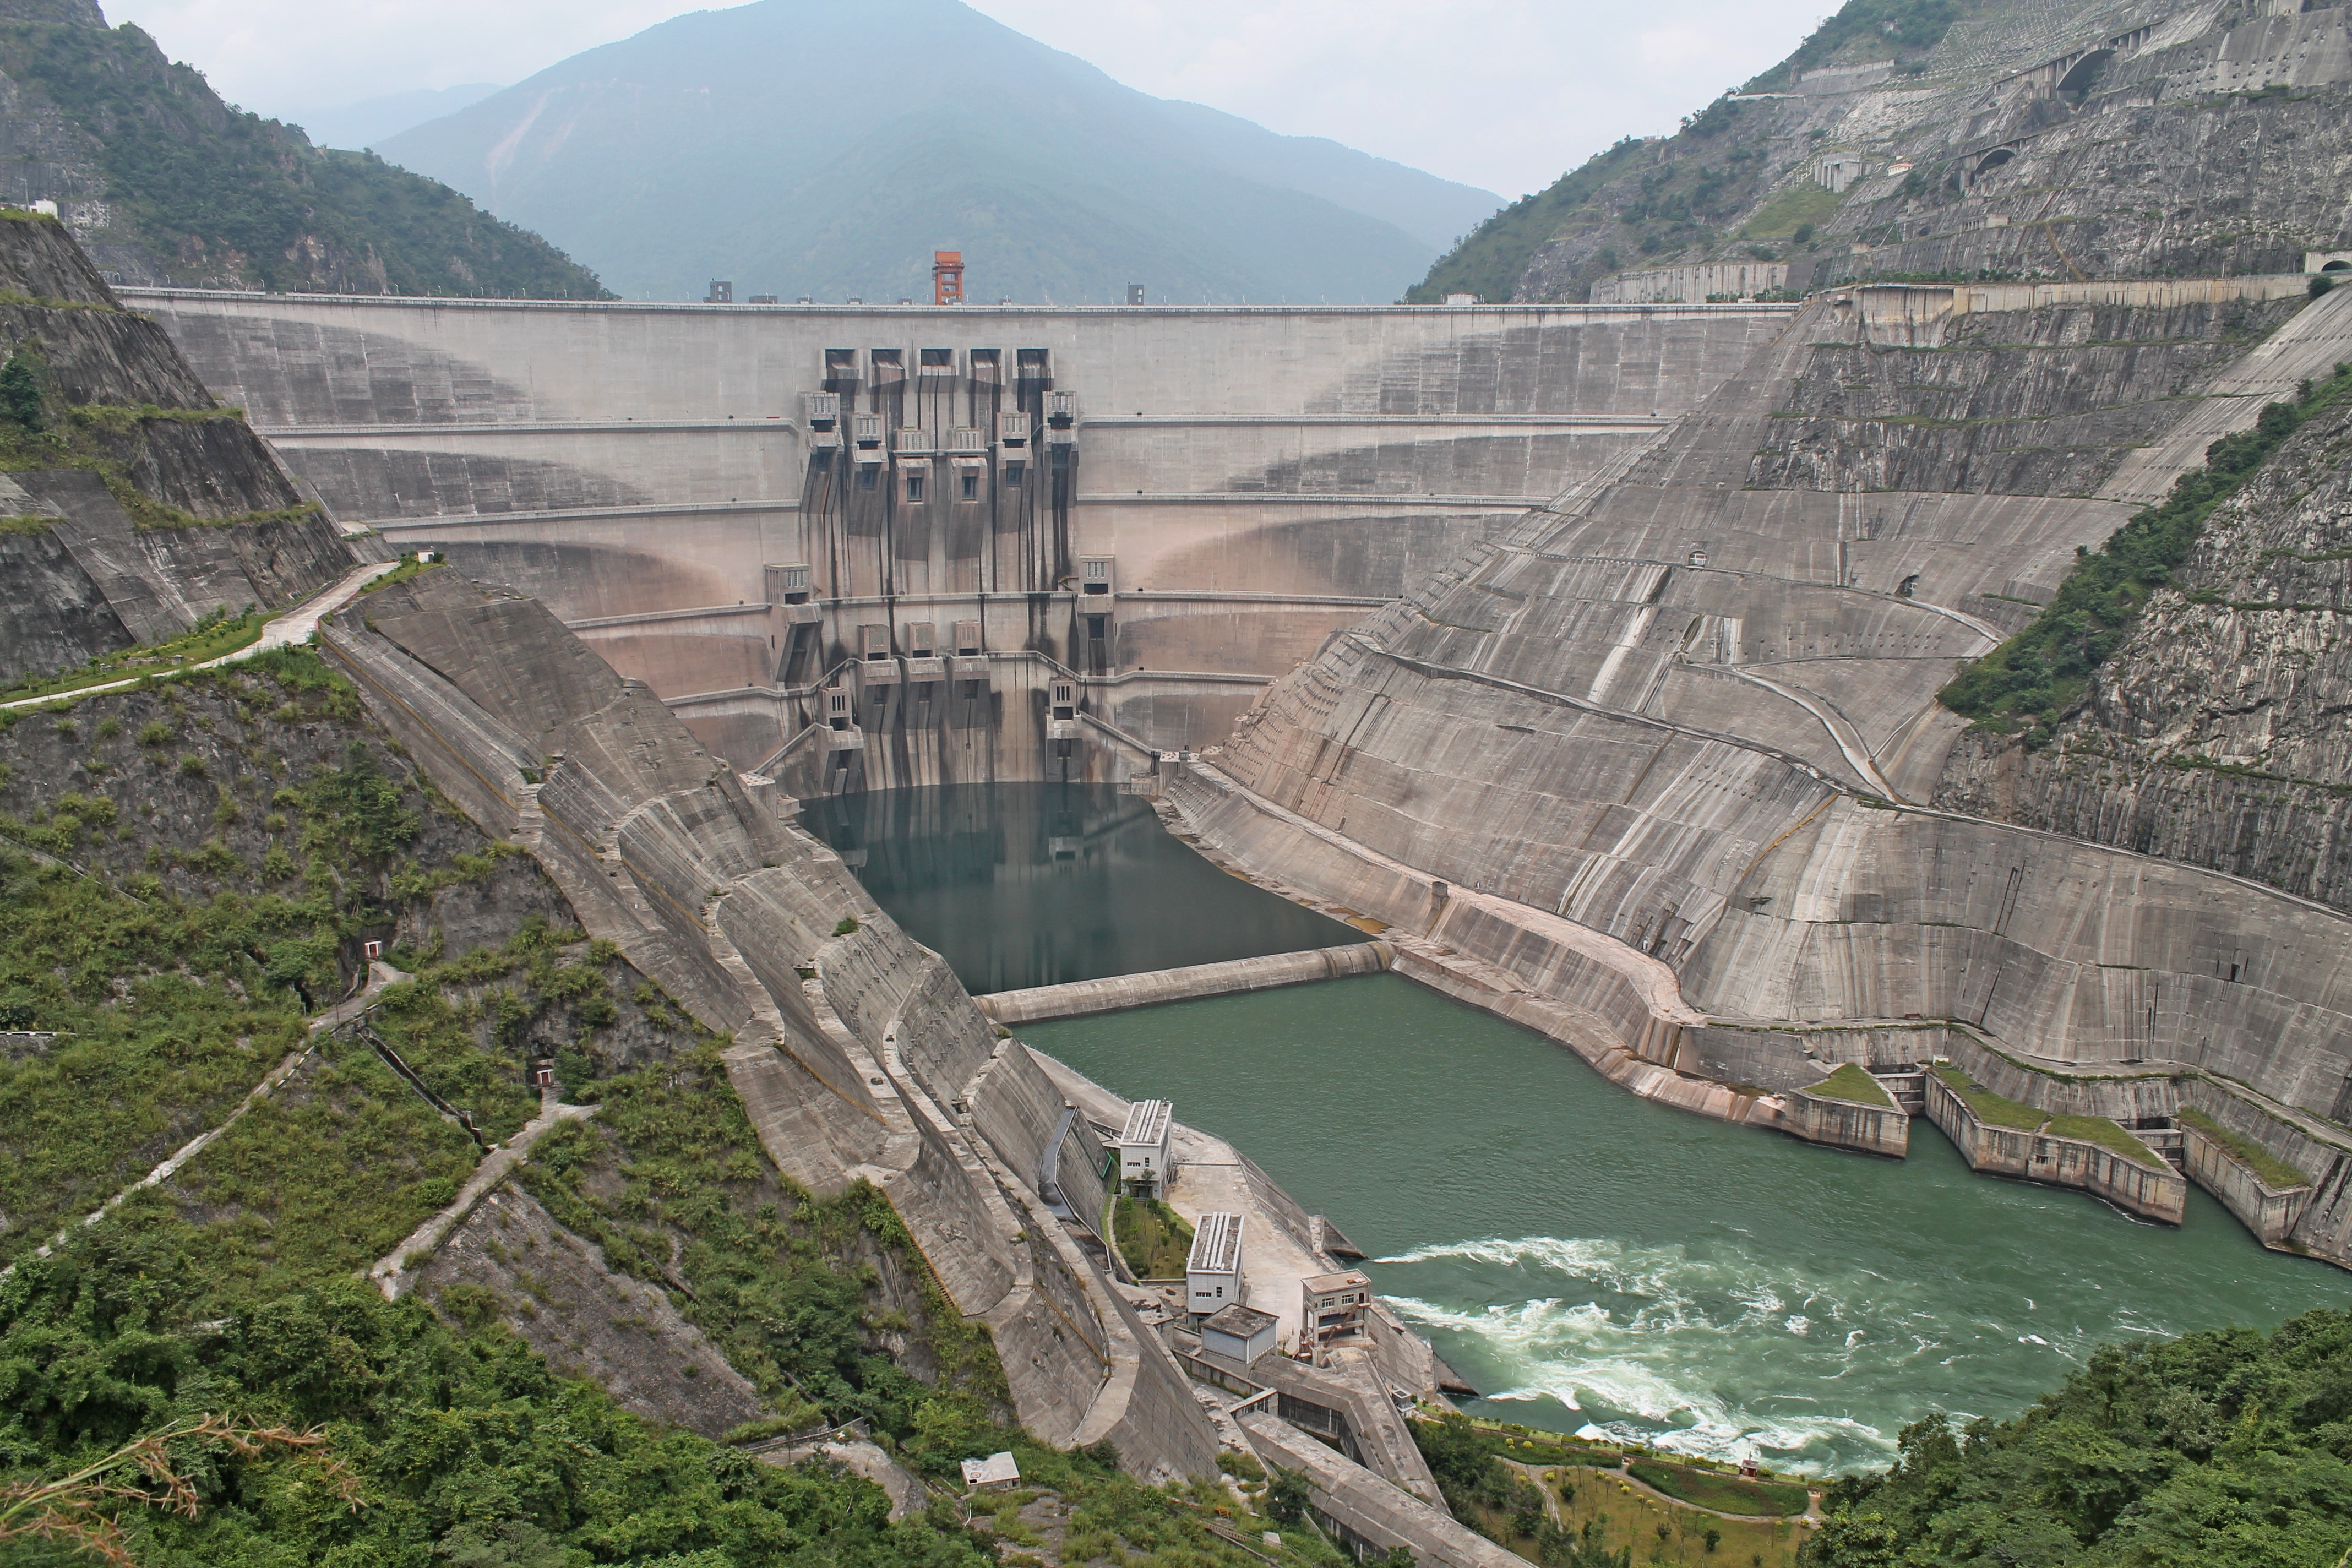
\includegraphics[scale=0.06]{mekong/02_dam.jpg}
\caption{Xiaowan Dam, Lancang (upper Mekong) River, China \cite{critnature}}
\end{figure}

Dams seem to cause a disturbance in the natural flow of the Mekong River, making both droughts and floods more common in the Mekong Delta. No constant stream of water upstream causes more saltwater intrusion downstream, making the agricultural industry less productive. Groundwater extraction causes subsidence, which in turn has very real consequences for the landscape of the delta.\\

\begin{figure}[h]
\centering
\includegraphics[scale=1]{mekong/01_groundwater.jpg}
\caption{Ground water treatment installation in Vietnam \cite{pernam}}
\end{figure}

As seen, the Mekong Delta's various sectors are facing numerous challenges, namely subsidence, salinization, and drought. These can be monitored by measuring variables such as conductivity, turbidity, and temperature continuously, across the Mekong River.


\newpage
\section{Related Studies}
In this section, an overview of current experience regarding water quality monitoring is given. This helps in identifying relevant theories, methods, and gaps in existing research.

\subsection{Indymo}
Indymo uses aquatic drones to collect underwater images, water samples and water quality and ecology data for public and private entities who want to inspect and monitor water systems. These drones are equipped with water quality sensors to collect data. Indymo has deployed their underwater drones in several countries such as the Netherlands, Vietnam, and Indonesia. \cite{indymoindonesia}

The primary purpose of these drones is to perform water quality mapping and monitoring of floating structures

As seen in an article published April 2020 \cite{indymoarticle}, Indymo tested multiple underwater drones (ROVs), each of them having with different characteristics. ROVs seem to have a generally a large payload capability which allows for bulky multi-parameter probes to be mounted on the ROV, probes normally used by hand.

\begin{figure}[h]
\centering
\includegraphics[scale=0.5]{similarprojects/11_innodrone.jpg}
\caption{Indymo's Innodrone (Based on the Thunder Tiger Neptune) \cite{indymoarticle}}
\end{figure}

They seem to measure water quality variables like pressure, temperature, conductivity, dissolved oxygen, algae and turbidity using one to two probes. Data was collected every 10s, and seem to be saved on the probes itself. Operational staff collected data simultaneously using conventional methods to validate the sensor data.

Indymo listed several multi-parameter probes they used throughout their research. They were very much of use as they gave insight as to what standards there are regarding water quality measurement precision.

\subsubsection{Similarity}
Indymo uses underwater ROVs for a 3D scan of the water, while this project focuses on using aerial UAVs to get a surface scan of the water. Both ways have its benefits and drawbacks, with Indymo's devices getting much more detailed information at the cost of man power and lack of automation.


\newpage
\subsection{Pelican Drone}
In September of 2019, the Micro Air Vehicle Lab of Delft University of Technology released a brief blog post about their developed "pelican drone" \cite{pelicandrone}. The pelican drone is capable of taking water samples quickly and analyse them in a CytoSense, a device that scans algae and other micro organisms. Taking water samples by hand is quite expensive and labour intensive. A drone speeds up this process significantly, allowing for more samples at less cost. 

MAVLab claims the drone is fitted with a hyperspectral camera to detect harmful algae, though the video \cite{pelicandronevideo} shows no hyperspectral camera fitted on the drone or hyperspectral images taken from the drone.\\

Looking closer at the drone, it seems to be a first generation Swellpro SplashDrone Marine Warrior \cite{marinewarrior}, with its built-in payload release system used for mounting the rope with sample tube.

\begin{figure}[h]
  \centering
  \begin{minipage}[b]{0.4\textwidth}
    \includegraphics[width=\textwidth]{similarprojects/21_marinewarrior.jpg}
    \caption{Swellpro SplashDrone Marine Warrior \cite{marinewarrior}}
  \end{minipage}
  \hfill
  \begin{minipage}[b]{0.5\textwidth}
    \includegraphics[width=\textwidth]{similarprojects/22_pelicandrone.jpg}
    \caption{TU Delft Pelican Drone \cite{pelicandrone}}
  \end{minipage}
\end{figure}

MAVLab states in the video and in the blog post that they were working on making the drone able to fly underwater.

Unfortunately, no further continuation of this project can be found. the initial blog post and video is all that is left. \cite{pelicandronevideo} 

\subsubsection{Similarity}
The pelican drone and this project both try to collect water samples using the drone. Where this project differs is that it also tries to measure multiple variables in real time using sensors.
\newpage
\subsection{Mapping water quality with drones: Test case in Texel} \label{similarprojects/multispectral}

As published in the IADC Dredging journal of December 2019, \cite{terraetaqua} a pilot test case at the Prins Hendrik Zanddijk project in Texel, The Netherlands, was organised to demonstrate drone technology for turbidity monitoring. An octocopter drone platform, Altura Zenith ATX8, was used with a multispectral camera, MicaSense RedEdge M, underneath.

The drone data was processed into turbidity maps. Water samples, collected simultaneously with drone flights were used for the validation of the sensor data.\\

The team noted that working with optical sensors add additional challenges. Water surfaces act as a mirror, and when sun light is reflected at the water surface, it is captured by the sensor. This results in a sun glints from which it is hard to obtain information on the water itself. Additionally, varying illumination conditions make it harder to quantify results.

\begin{figure}[h]
\centering
\includegraphics[scale=1]{similarprojects/31_uncorrected.png}
\caption{Uncorrected image with sun glint \cite{terraetaqua}}
\end{figure}

As shown in the publication, some of these problems can be mitigated by slightly tilting the camera and creating flight plans which look away from the sun. The remaining artifacts can be filtered out by an image processing chain.

The results of the pilot test case was positive, with the turbidity values obtained from the drone imagery being within range of manual measurements, though the validation dataset available is pretty small.

The authors stated that in the future, a semi-autonomous data collection architecture can be made where a drone can be triggered by other sensors when these sensors detect an anomaly, performing a defined flight mission.

\subsection{Similarity}
While this project may make use of optical sensors for the assessment of water quality, both projects definitely do have aspirations of being autonomously monitored. The test case opted for a non-waterproof octocopter as the UAV doesn't have to land in the water.
\newpage
\section{Water Quality Parameters} \label{variables}
In this section, multiple water quality parameters are described. A combination of these known parameters help with the evaluation of the total water quality in respect to different water applications such as surface water treatment and irrigation.

A small description of every parameter will be given, after which some sensors that may be suitable for mounting on the drone will be reviewed. Some multi parameter sensor systems will also be reviewed. In the following design report, a practical stack of some sensors will be made

%
%\subsection{Variables} 

%What are some useful things to know before surface water treatment?
%What is considered acceptable irrigation water?

%In the drone
\subsection{Temperature}
Temperature readings are used in the calculation of acidity, salinity, and in colorimetric tests. In limnological studies, knowledge of water temperatures as a function of depth often are required. The source of water supply, such as deep wells, often can be identified by temperature measurements alone. Surface water treatment plants also require data on water temperature at intake, as the viscosity of the water can differ. \cite{standardmethods}

\subsubsection{Sensors}
In this section, a comparison between potential temperature (℃) sensors for the project is given. Certain features like price, accuracy, and form factor will be given. The temperature sensors selected can be submerged in water.

\paragraph{DFRobot DFR0198/DS18B20}\mbox{€6,31} \cite{DFR0198}
\begin{table}[h!]
	\centering
	\adjustimage{height=4cm,valign=c}{water/41_dfr0198.jpg}\quad
	\begin{tabular}{| l | l |}
    \hline
    Protocol & 1-Wire\\
    Measurement Range & -10-85 ℃ \\
    Measurement Accuracy &  0.5 ℃ \\
    Response time & Within 750ms \\
    Supply Voltage & 3.3V-5V \\
    Software library included & yes \\
    Availability & 3-5 Working Days \\
    \hline
	\end{tabular}
\end{table}

\paragraph{Littelfuse USP10982}\mbox{€3,48} \cite{USP10982}
\begin{table}[h!]
	\centering
	\adjustimage{height=4cm,valign=c}{water/42_usp10982.jpg}\quad
	\begin{tabular}{| l | l |}
    \hline
    Protocol & Resistance (Analog)\\
    Measurement Range & 25-80 ℃ \\
    Measurement Accuracy &  0.55 ℃ after calibration\\
    Response time & Within 15s \\
    Software library included & no \\
    Availability & 3-5 Working Days \\
    \hline
	\end{tabular}
\end{table}
%In the drone
\newpage
\subsection{Acidity} \label{acidity}
Acidity is the quantitative capacity of a water or solution to neutralize an alkali. pH is a measure of the acidity or basicity of an aqueous solution. Solutions with a pH less than 7 are said to be acidic and solutions with a pH greater than 7 are basic or alkaline. \cite{phmerriam} Acidity can be interpreted in terms of specific substances only when the chemical composition of the sample is known. In this section, a closer look is taken at pH and how it affects the water quality. 

\subsubsection{Temperature}
The pH is inversely proportional to the temperature of the solution. When the temperature of a solution rises, the molecular vibrations in the solution rise resulting in the ionization and formation of H+ ions. More H+ ions lead to more acidic behavior. Generally, if we increase the temperature by 10°C, the pH of a solution or a substance will drop by 0.2.  \cite{temperatureph}

\subsubsection{Corrosion}
The pH is inversely proportional to the rate of corrosion. Corrosion occurs due to the formation of electrochemical cells. Low pH acid waters accelerate corrosion by providing a plentiful supply of hydrogen ions. The metal acts like an anode, with more negative potential with respect to the water which acts like a cathode. \cite{standardmethods}

\subsubsection{The carbon dioxide equilibrium system}
One of the most important chemical properties of water is that it can be both an acid and a base, because water ionizes into H+ and OH- ions.
The ionization is an equilibrium reaction.\\
The concentration of $H^+$ is usually denoted as the negative logarithm pH, while the concentration of $OH^-$ is denoted as the negative logarithm pOH.
For a neutral solution with a pH/pOH of 7.0 at 25 degrees celsius:
\[H^+ = OH^- = 0.0001 mmol/L\]
A lower pH than 7.0, meaning a higher concentration of H+ ions, indicates an acid solution. Water with a pH above 7 is a base. The pH of most raw water lies within the range 6.5–8.5 \cite{standardmethods}\\

The most important acid-base reaction in water is related to the dissociation of carbon dioxide. \cite{aes} When $CO_2$ becomes aqueous in water, a small portion of it becomes $H_2CO_3$, leaving $H^+$ ions:
\[CO_2 + H^2O <=> H^+ + HCO_3\]
$HCO_3^-$ can at it's turn release another $H^+$ ion:
\[HCO_3^- <=> CO_3^{2-} + H^+\]
The amount of carbon dioxide $CO_2$ in solution can determine the pH of the water. The most common source of acidity in water is dissolved $CO_2$, so the more $CO_2$ in the water, the lower the pH. As seen, dissolved $CO_2$ undergoes different stages over time. These stages have different pH levels associated with them:

\begin{figure}[h]
\centering
\includegraphics[scale=0.9]{water/21_equilibrium.jpg}
\caption{pH/$CO_2$ equilibrium \cite{aes}}
\end{figure}

\newpage
\subsubsection{Sensors}
In this section, a comparison between potential acidity (pH) sensors for the project is given. Certain features like price, accuracy, and form factor will be given.

To ensure accuracy, a pH probe needs to be calibrated first in two buffer solutions, pH 4.0 and pH 7.0. This has to be done every month. These buffer solutions usually cost around €15,- or can be found in most chemistry labs. As the pH is inversely proportional to the temperature of the solution, one should also use a temperature sensor to get meaningful data.

\paragraph{DFRobot Gravity V2}\mbox{€35.92} \cite{SEN0161V2}
\begin{table}[h!]
	\centering
	\adjustimage{height=4cm,valign=c}{water/22_gravityv2.jpg}\quad
	\begin{tabular}{| l | l |}
    \hline
    Interface & Analog \\
    Measurement Range & 0-14 pH \\
    Measurement Accuracy &  0.1pH \\
    Response time & Within 2min \\
    Supply Voltage & 3.3V-5V \\
    Software library included & yes \\
    Long term immersion & no \\
    Availability & 3-5 Working Days \\
    \hline
	\end{tabular}
\end{table}

\newpage
\paragraph{DFRobot Gravity V2 Pro}\mbox{€59,01} \cite{SEN0169V2}
\begin{table}[h!]
	\centering
	\adjustimage{height=4cm,valign=c}{water/23_gravityv2pro.jpg}\quad
	\begin{tabular}{| l | l |}
    \hline
    Interface & Analog \\
    Measurement Range & 0-14 pH \\
    Measurement Accuracy &  0.1pH \\
    Response time & Within 1min \\
    Supply Voltage & 3.3V-5V \\
    Software library included & yes \\
    Long term immersion & yes \\
    Availability & 3-5 Working Days \\
    \hline
	\end{tabular}
\end{table}


\paragraph{Generic PH0-14}\mbox{€15,83} \cite{PH0-14}
\begin{table}[h!]
	\centering
	\adjustimage{height=4cm,valign=c}{water/24_ph014.jpg}\quad
	\begin{tabular}{| l | l |}
    \hline
    Interface & Analog \\
    Measurement Range & 0-14 pH \\
    Measurement Accuracy &  0.25pH \\
    Response time & Within 1min \\
    Supply Voltage & 3.3V-5V \\
    Software library included & no \\
    Long term immersion & no \\
    Availability & 26 Days \\
    \hline
	\end{tabular}
\end{table}



\newpage
\subsection{Alkalinity}
Total alkalinity is a measurement of the water’s ability to resist a reduction in pH. Alkalinity ions resist reduction in pH by attracting a Hydrogen ion if needed. Total alkalinity is measured by the concentration (parts per million) in the water. \cite{standardmethods} In this section, a closer look is taken at total alkalinity and how it affects the water quality in different scenario's.

\subsubsection{Irrigation Water}
In order to evaluate the quality of irrigation water, one should know both pH and alkalinity. A pH test by itself is not an indication of alkalinity. Water with high alkalinity always has a pH value 7 or above, but water with high pH doesn't always have high alkalinity. 

Irrigating with water having a high pH causes no problems as long as the alkalinity is low (0 to 100 ppm calcium carbonate). The irrigation water will probably have little effect on growing medium pH because it has little ability to neutralize acidity.

Problems occur when water that has both high pH and high alkalinity is used for irrigation. The pH of the growing medium may increase significantly with time, decreasing crop rates. It is much more difficult to predict the effects of irrigating outdoor flower crops, gardens, and landscape plants with water having high pH and high alkalinity. 

Moderately alkaline water could be beneficial however as a source of extra $Ca$ and $Mg$ for crops prone to $Ca$ and $Mg$ deficiencies \cite{umassalkalinity}

\subsubsection{Water for aquatic life}
Fish and other aquatic life generally need a pH range of 6.5 to 8.0. \cite{fishphghkh} Since alkalinity buffers against rapid pH changes, the alkalinity helps protect the living organisms who need a specific pH range. Higher alkalinity levels in surface water can buffer acid rain and other acid wastes. This can prevent pH changes that are hazardous to aquatic life. 

%For drinking water?

\subsubsection{Sensors}

While there does exist a total alkalinity (ppm) sensor, it exists in the form of a lab-on-chip prototype developed by the national oceanography centre. \cite{alkalinitysensor} It is a bulky 6kg device meant to be used in large ships, and in no form suitable to be deployed in this project.

\paragraph{Lab-on-Chip Total Alkalinity Sensor}\mbox{} \cite{alkalinitysensor}
\begin{table}[h!]
	\centering
	\adjustimage{height=4cm,valign=c}{water/31_alkalinitysensor.jpg}\quad
	\begin{tabular}{| l | l |}
    \hline
    Measurement Range & 600umol/kg \\
    Measurement Accuracy &  5 umol/kg \\
    Response time & 12 min \\
    Supply Voltage & 10-16V \\
    Weight & 6kg \\
    Availability & Unknown \\
    \hline
	\end{tabular}
\end{table}

\newpage
%In the drone
\subsection{Conductivity}
Conductivity of a substance is defined as 'the ability or power to conduct or transmit heat, electricity, or sound'. \cite{merriamconductivity} Its units are Siemens per meter [S/m] in SI. Electrical conductivity is defined as the ratio between the current density (J) and the electric field intensity (e) and it is the reciprocal of the resistance:

\[s = J/e = 1/r\]

In water and ionic materials or fluids a net motion of charged ions can occur. This phenomenon produce an electric current and is called ionic conduction. Pure water is not a good conductor of electricity. Because the electrical current is transported by the ions in solution, the conductivity increases as the concentration of ions increases. \cite{lenntech} Conductance in water also depend on the mobility of the ions, the valence, and the temperature of the substance. \cite{standardmethods}\\


\subsubsection{Salinity}
In natural water, salinity is often determined by measuring the conductivity of the water. Typical values go as follows:

\begin{figure}[h]
\centering
\includegraphics[scale=0.4]{water/61_typicalvalues.png}
\caption{Typical resistivity, conductivity and salinity values for different types of water \cite{abdulsamsudin}}
\end{figure}

\newpage
\subsubsection{Sensors}
In this section, a comparison between potential conductivity sensors for the project is given. Certain features like price, accuracy, and form factor will be given.

To ensure accuracy, a conductivity probe needs to be calibrated first in two buffer solutions of 1413us/cm and 12.88ms/cm. \cite{DFR0300H} This has to be done every month. These buffer solutions usually cost around €13,- or can be found in most chemistry labs.

\paragraph{Analog Devices EVAL-CN0349-PMDZ}\mbox{€49,04} \cite{CN0349}
\begin{table}[h!]
	\centering
	\adjustimage{height=4cm,valign=c}{water/62_cn0349.jpg}\quad
	\begin{tabular}{| l | l |}
    \hline
    Protocol & I2C\\
    Measurement Accuracy &  1\% FSR\\
    Supply Voltage & 3.3V\\
    Software library included & no \\
    Probe included & yes \\
    Availability & 2 Months \\
    \hline
	\end{tabular}
\end{table}

\paragraph{Gravity: Analog Electrical Conductivity Sensor}\mbox{€72,70} \cite{DFR0300H}
\begin{table}[h!]
	\centering
	\adjustimage{height=4cm,valign=c}{water/63_dfr0300h.jpg}\quad
	\begin{tabular}{| l | l |}
    \hline
    Protocol & Analog\\
    Measurement Accuracy &  5\% FSR\\
    Supply Voltage & 3.3-5V\\
    Support Detection Range & 10~100ms/cm\\
    Software library included & yes \\
    Probe included & yes \\
    Availability & 3-5 Working days \\
    \hline
	\end{tabular}
\end{table}
%In the drone
\newpage
\subsection{Turbidity}
Turbidity in water is caused by suspended and colloidal matter such as clay, silt, finely divided organic and inorganic matter, plankton and other microscopic organisms. Turbidity is an expression of the optical property that causes light to be scattered and absorbed rather than transmitted with no change in direction or flux level through the sample. \cite{standardmethods}\\

The unit measuring turbidity is known as NTU or JTU (Jackson Turbidity Unit):

\[1JTU = 1NTU = 1 mg/L\]


Clarity of water is important in producing products destined for human consumption and in many manufacturing operations. \cite{standardmethods} Water treatment plants drawing from a surface water source commonly rely on fluid-particle separation processes such as sedimentation and filtration to increase clarity and ensure an acceptable product.\\


\subsubsection{For aquatic life}

The clarity of a natural body of water is an important determinant of its productivity. Light penetration is especially important for submerged aquatic plants. These plants depend on light interception and absorption for photosynthesis. Enough light must be absorbed by the plant for photosynthesis to result in a net increase in biomass in order for the plant to grow and reproduce. 

Too much reductions in light levels result in death of the plant. As a result, plant growth in waters containing much turbidity and color is typically restricted to shallow depths, whereas plant growth is less restricted in less-turbid water. Submerged aquatic vegetation is a very important component of aquatic ecosystems. It provides food, shelter, and protection for many different aquatic species. Declines in this habitat will indirectly affect populations of species that depend on it. \cite{standardmethods}

\subsubsection{Using a multispectral camera}
As seen in \ref{similarprojects/multispectral} it is possible to get turbidity estimates by using a multispectral camera. This has the benefit of being able to cover a great amount of data in a short amount of time. It does require a lot of additional post processing to get realistic turbidity maps.

\subsubsection{Using a secchi disk}
A Secchi disk is a 30 cm disk with alternating black and white quadrants. It is lowered into the water until it can no longer be seen by the observer. This depth of disappearance, called the Secchi depth, is a measure of the transparency of the water. On an UAV, one could possibly use a RGB camera, a hoist, and machine vision to determine when the secchi depth is reached. \cite{secchidisk}

\newpage
\subsubsection{Sensors}
In this section, a comparison between potential turbidity sensors for the project is given. Certain features like price, accuracy, and form factor will be given.

As turbidity levels can change given depth, one should look into lowering these sensors at different depths.

\paragraph{DFRobot SEN0189}\mbox{€9.01} \cite{SEN0189}
\begin{table}[h!]
	\centering
	\adjustimage{height=4cm,valign=c}{water/71_sen0189.jpg}\quad
	\begin{tabular}{| l | l |}
    \hline
    Protocol & Analog\\
    Operating Temperature & 5-90 ℃ \\
    Operating Range &  0-3000NTU\\
    Response time & Within 500ms \\
    Supply Voltage & 0V-4.5V \\
    Software library included & yes \\
    Availability & 3-5 Days \\
    \hline
	\end{tabular}
\end{table}

\paragraph{Keyeyestudio KS0414}\mbox{€12.72} \cite{KS0414}
\begin{table}[h!]
	\centering
	\adjustimage{height=4cm,valign=c}{water/72_ks0414.png}\quad
	\begin{tabular}{| l | l |}
    \hline
    Protocol & Analog\\
    Operating Voltage & 5V\\
    Opearting Temperature & -30℃-80℃\\
    Operating Range & 0-4550NTU\\
    Measurement Accuracy & 228NTU\\
    Response time & Within 500ms \\
    Supply Voltage & 0V-4.5V \\
    Software library included & no \\
    Availability & 2 Weeks \\
    \hline
	\end{tabular}
\end{table}


\newpage
\subsection{Oxidation-Reduction Potential}
To reach a state of stability, substances that are lacking electrons are desperately seeking out electrons wherever they can. On the contrary, substances which have a surplus of electrons are capable of donating their extra electrons. These are called oxidizing and anti-oxidizing agents respectively.\\

Oxidation-reduction potential, or ORP, is a measurement that indicates the degree to which a substance is capable of oxidizing or reducing another substance. ORP is measured in millivolts.\cite{phorp} If the pH of water is higher than 9.5, then ORP meters become an invalid method of water quality measurement. \cite{standardmethods}

\subsubsection{Use in water treatment systems}
Water treatment is often accomplished through the addition of chlorine. The resulting oxidation reaction with water forms hypochlorous acid. In water treatment applications ORP is used to measure the oxidation by controlling the amount of free chlorine until a known bacteria killing ORP level is achieved. \cite{hamilton}

\subsubsection{Sensors}
In this section, a comparison between potential ORP sensors for the project is given. Certain features like price, accuracy, and form factor will be given.

\paragraph{DFRobot SEN0165}\mbox{€83,04} \cite{SEN0165}
\begin{table}[h!]
	\centering
	\adjustimage{height=4cm,valign=c}{water/81_sen0165.jpg}\quad
	\begin{tabular}{| l | l |}
    \hline
    Protocol & Analog\\
    Operating Temperature & 5-70 ℃ \\
    Operating Range &  -2000mV—2000mV\\
    Measurement Accuracy &  10mV \\
    Response time & Within 20s \\
    Supply Voltage & 5V \\
    Software library included & yes \\
    Availability & 3-5 Days \\
    \hline
	\end{tabular}
\end{table}

\paragraph{Generic ORP Sensor}\mbox{€50,58} \cite{orpsensor}
\begin{table}[h!]
	\centering
	\adjustimage{height=4cm,valign=c}{water/82_orpsensor.jpg}\quad
	\begin{tabular}{| l | l |}
    \hline
    Protocol & Analog\\
    Operating Temperature & 5-70 ℃ \\
    Operating Range &  -2000mV—2000mV\\
    Measurement Accuracy &  10mV \\
    Response time & Within 1min \\
    Supply Voltage & 5V \\
    Software library included & yes \\
    Availability & 26 Days \\
    \hline
	\end{tabular}
\end{table}
%Optionally in the drone
\newpage
\subsection{Total Dissolved Solids}
Total dissolved solids (TDS) can be defined as the mass of residue remaining when a measured volume of filtered water is evaporated. TDS is usually written in ppm (parts per million).

While turbidity is about particles that are not dissolved in water, total dissolved solids are about particles that are totally dissolved in water. TDS is usually low for freshwater sources, at less than 500 ppm. Seawater contains about 500-30,000 ppm, while brackish water contains 30–40,000 ppm.

\begin{figure}[h]
\centering
\includegraphics[scale=0.69]{water/91_tdschart.jpg}
\caption{TDS Chart for drinking water\cite{tdschart}}
\end{figure}

%Difference between conductivity sensor and tds sensor


\subsubsection{Sensors}
TDS sensors generally require temperature compensation in order to give accurate readings. Lower end models also generally require calibration from first use using a buffer solution of a known parts per million substance. \cite{sen0244wiki}

\paragraph{DFRobot SEN0244}\mbox{€11,66} \cite{SEN0244}
\begin{table}[h!]
	\centering
	\adjustimage{height=4cm,valign=c}{water/92_sen0244.jpg}\quad
	\begin{tabular}{| l | l |}
    \hline
    Protocol & Analog\\
    Operating Range & 0 ~ 1000ppm\\
    Measurement Accuracy &  100ppm \\
    Response time & Unknown \\
    Supply Voltage & 3.3V-5V \\
    Software library included & yes \\
    Availability & 3-5 Days \\
    \hline
	\end{tabular}
\end{table}

\newpage
\subsection{Multiparameter meter}
Multiparameter meters are instruments used to measure multiple electrochemical parameters at once. These may include methods for acidity, temperature, conductivity, turbidity, ORP, TDS, and more. All of the selected multiparameter meters are suitable for continuous testing in natural waters.

\paragraph{Aquaread AP2000}\mbox{} \cite{AP2000}
\begin{table}[h!]
	\centering
	\adjustimage{height=3cm,valign=c}{water/101_ap2000.jpg}\quad
	\begin{tabular}{| l | l | l |}
    \hline
    Variable & Range & Accuracy\\
    \hline
    DO & 0 – 50.00 mg/L & 0.01mg/L\\
    ORP & -2000 - 2000mV & 5mV\\
    Conductivity & 0 – 200mS/cm & 1\% FSR\\
    Acidity & 0 – 14pH & 0.01pH\\
    Temperature & -5C – +50C & 0.5C\\
    \hline
	\end{tabular}
\end{table}
\\The AP2000 can be fitted with additional optical or ion selective sensors to sense specific substances such as refined oil or ammonium. Values are saved on a standalone meter. One can retrieve sensor data from this meter and export it to CSV via a proprietary Windows application. It has a weight of 700g, excluding the meter.

\paragraph{PME Minidot}\mbox{} \cite{minidot}
\begin{table}[h!]
	\centering
	\adjustimage{height=3cm,valign=c}{water/102_minidot.jpg}\quad
	\begin{tabular}{| l | l | l |}
    \hline
    Variable & Range & Accuracy\\
    \hline
    DO & 0 – 50.00 mg/L & 0.3mg/L\\
    Temperature & 0C - 35C & 0.1C\\
    \hline
	\end{tabular}
\end{table}
\\One can retrieve real-time data from the logger via serial communication. The Minidot has a weight of 340g.

\paragraph{van Essen CTD Diver}\mbox{} \cite{ctddiver}
\begin{table}[h!]
	\centering
	\adjustimage{height=4cm,valign=c}{water/104_troll9500.png}\quad
	\begin{tabular}{| l | l | l |}
    \hline
    Variable & Range & Accuracy\\
    \hline
    Conductivity & 0 – 120 mS & 1\% FSR\\
    Temperature & 0C - 35C & 0.1C\\
    \hline
	\end{tabular}
\end{table}
\\After measurements, one can retrieve data from the logger via the included proprietary interface cable and Windows software. The CTD Diver has a weight of 95g.
\newpage
\paragraph{In-Situ TROLL 9500 Professional}\mbox{} \cite{AP2000}
\begin{table}[h!]
	\centering
	\adjustimage{height=3cm,valign=c}{water/101_ap2000.jpg}\quad
	\begin{tabular}{| l | l | l |}
    \hline
    Variable & Range & Accuracy\\
    \hline
    DO & 0-20-50 mg/L & 0.01-0.02-0.5mg/L\\
    ORP & -1400 - 1400mV & 5mV\\
    Conductivity & 0 – 200mS/cm & 0.5\% FSR\\
    Acidity & 0 – 12pH & 0.01pH\\
    Temperature & -5C – +50C & 0.5C\\
    \hline
	\end{tabular}
\end{table}
\\The TROLL 9500 is available in multiple editions with additional optical or ion selective sensors to sense specific substances such as ammonium, chloride, nitrate, and turbidity. Values are transmitted via the RS485/RS232 serial protocol. It has a weight of 1.9kg.
\newpage
\section{UAV}
In this section, a comparison between potential drone models for the project is given. The possibility of a DIY Drone will be reviewed, and the basic theory of a mounting solution will be discussed.

\subsection{Existing Models}
Necessary requirements are elaborated and graded on every drone. As this comparison is purely about the performance of the drone for the project, no attention is given to price until after this comparison. Options for acquiring the drone will be briefly discussed.

\subsubsection{Grading} \label{grading}
Drones are graded by a product of their requirements. They start out with a score of 1. Each of these requirements are graded by rational number from 0-1.5. This way, a requirement score of 1.2 can positively affect the end grade, while a requirement score of 0 dismisses the drone all together. 

This makes it possible to easily disregard a drone when it does not meet a requirement at all. Care must be put in dismissing drones though, since there sometimes exist alternatives that can fix these requirements. Generally, any drone above a score of 1 can be suitable for the project. 

\subsubsection{Overview of the requirements}
In this section, an overview of the requirements are given, including minimal values for these requirements. Further explanation might be given about different solutions that might exist to reach these requirements. 

\paragraph{Payload capacity}\mbox{} \\
The payload capacity is the maximum amount of weight a drone can safely carry while flying. While exceeding the payload capacity by a bit is often possible, it is never encouraged by the manufacturer. A large payload can shift the center of mass too much for the drone's stabilization to work reliably. There are also physical limits to the combined lifting force of the rotors. Summing up the weight of potential sensors of the drone, it is expected that the minimum payload capacity on paper should be 500g.

\paragraph{Mounting clearance}\mbox{} \\
There are several ways to mount sensors on a drone. Some drones have dedicated mounting holes while others rely on the user to come up with their own solution. There must be enough clearance on the bottom of the drone for the sensors to mount on. The amount of clearance could sometimes be extended by modifying the drone.

\paragraph{Navigation/Routing}\mbox{} \\
The drone must be able to navigate on its own to multiple previously marked GPS locations and return to home. Some drones have this functionality built into their own app, others don't even have an app. When this functionality isn't built in, it could be developed or the drone could be integrated into an open source software suite like ArduPilot \cite{ardupilot} if a SDK is available. This would delay the development cycle.
\newpage
\paragraph{Flight time}\mbox{} \\
The drone ideally should be able to take multiple measurements per flight. Care should be taken when looking at flight times at data sheets, as these often don't include flight time whenever the drone has payload. The longer the flight time the better, a minimum of 10 minutes flight time should be fine.

\paragraph{Range}\mbox{} \\
Often there are two different ranges included in datasheets, the image transmission range and the drone operating radio range. In this project, real time transmission of images has a low priority, so the focus is laid on operating radio range. Again, care should be taken whenever looking at range as data sheets usually report this range without obstructions. Thankfully, as there are little obstructions in the Mekong Delta, the realistic range would be very similar. A minimum of 1 kilometer operating range is required.

\paragraph{Waterproof}\mbox{} \\
It is important to reduce the risk of damaging the drone as much as possible. As the measurements takes place near and on water, using a waterproof drone is vital. Generally, drones denote the level of solid and liquid protection by the Ingress Protection standard. The IP standard classifies the degree of protection provided by an enclosure. \cite{ipstandard} For this project, a minimum rating of IP64 would be sufficient, meaning dust-tight and resistant against splashes of water.

For drones that are not waterproof, certain wet suits are available to alleviate this issue. \cite{phantomrain}

\paragraph{Landing in water}\mbox{} \\
For some measurements and emergency landings it is best that the drone is able to land in the water. While there are not a lot of drones available that have this feature out of the box, there is some commercial water landing gear available.\cite{buylanding} Designing your own landing gear is also possible. \cite{diylanding} Water landing gear often also increase the amount of clearance available for sensors.

\paragraph{Maneuverability}\mbox{} \\
The drone should not get stuck on it's flight in the Mekong River. It should be fast enough to take the measurements, and it should be stable enough to be used in an autonomous environment. These aspects are what determines the maneuverability of the drone.

\newpage
\subsubsection{Swellpro SplashDrone 4}
\begin{wrapfigure}{r}{0.3\textwidth}
\includegraphics[width=1\linewidth]{uav/models/01_splashdrone4.png}
\caption{SplashDrone 4}
\end{wrapfigure}
The SplashDrone 4 \cite{splashdrone4} is Swellpro's flagship drone. It is fully designed to be used in the water.

\paragraph{Payload capacity}\mbox{Score: 1.5} \\
The payload capacity of the SplashDrone 4 is 2kg, enough for all of our gear.

\paragraph{Mounting clearance}\mbox{Score: 1.3} \\
The SplashDrone 4 is a medium compact drone and therefore doesn't have a lot of clearance for sensors. It does have mounting holes for payloads at the bottom of the drone, which make mounting sensors easy. The drone can also flip over in the water, so one could also manually mount sensors on top of the drone. Additionally, Swellpro sells a water collector for the Splashdrone 4 to take water samples. \cite{watercollector}

\paragraph{Navigation/Routing}\mbox{Score: 1.5} \\
One can plan routes for the SplashDrone 4 using the SwellPro SDFly App. The app has support for waypoint mission planning and grid mission planning. Additionally, a SDK and API is also in development for when one wants to create their own add-ons or flight platform.

\paragraph{Flight time}\mbox{Score: 1.5} \\
The flight time of the SplashDrone 4 is 30 minutes, well over the minimum required flight time.

\paragraph{Range}\mbox{Score: 1.5} \\
The maximum radio range is 5.0km, well over the minimum required range. This also includes image transmission.

\paragraph{Waterproof}\mbox{Score: 1.5} \\
The drone is IP67 waterproof, meaning the drone is dust-tight and can immerse up to 1 meter in water. This is well over the minimum required IP rating.

\paragraph{Landing in water}\mbox{Score: 1.5} \\
The drone is designed to land and take off in the water.

\paragraph{Maneuverability}\mbox{Score: 1.4} \\
When the drone turns upside down on the water for any reason, it automatically turns the drone back around to the normal state. It can fly horizontally 10m/s with the GPS being the limiting factor.

\paragraph{Total score:}\mbox{20.7} \\
The SplashDrone 4 seems to be a very adequate system for the project, with it's extensible and water-first design.
\newpage
\subsubsection{Swellpro Fisherman FD1}
\begin{wrapfigure}{r}{0.3\textwidth}
\includegraphics[width=1\linewidth]{uav/models/11_fishermanfd1.png}
\caption{Fisherman FD1}
\end{wrapfigure}
The Fisherman FD1 \cite{fishermanfd1} is Swellpro's economical offering based on their previous flagship. It is also fully designed to be used in the water.

\paragraph{Payload capacity}\mbox{Score: 1.5} \\
The payload capacity of the Fisherman FD1 is 2kg, well above the minimum requirement.

\paragraph{Mounting clearance}\mbox{Score: 1.1} \\
The Fisherman FD1 is a medium compact drone and therefore doesn't have a lot of clearance for sensors. One could create their own platform beneath the drone, utilizing the four feet.

\paragraph{Navigation/Routing}\mbox{Score: 0.5} \\
While the Fisherman FD1 is based off of the SplashDrone 3+ that has an app that allows waypoints, it is not clear if this revised version can use that app as well. One might need to acquire a remote from the SplashDrone 3+ for the app to work.
As an alternative, one could hack into the internals of the drone with relative ease and use an open source flight system like ArduPilot.

\paragraph{Flight time}\mbox{Score: 1.5} \\
The flight time of the SplashDrone 4 is 30 minutes, well over the minimum required flight time.

\paragraph{Range}\mbox{Score: 1.2} \\
The maximum radio range is 1.6km, passing the minimum required range. This includes image transmission.

\paragraph{Waterproof}\mbox{Score: 1.5} \\
The drone is IP67 waterproof, meaning the drone is dust-tight and can immerse up to 1 meter in water. This is well over the minimum required IP rating.

\paragraph{Landing in water}\mbox{Score: 1.5} \\
The drone is designed to land and take off in the water.

\paragraph{Maneuverability}\mbox{Score: 1.1} \\
The drone can fly horizontally 10m/s with the GPS being the limiting factor.

\paragraph{Total score:}\mbox{3.7} \\
The Fisherman FD1 looks like a capable budget-friendly alternative to the SplashDrone 4, but the compatibility of the waypoint app needs to be figured out.


\newpage
\subsubsection{Swellpro Spry+}
\begin{wrapfigure}{r}{0.3\textwidth}
\includegraphics[width=1\linewidth]{uav/models/21_spry.png}
\caption{Spry+}
\end{wrapfigure}
The Spry+ \cite{spry} is Swellpro's action drone. It is also fully designed to be used in the water.

\paragraph{Payload capacity}\mbox{Score: 0} \\
While the payload capacity of the Spry+ is not presented on the website, professionals state that the drone can carry up to 300g\cite{sprypayload}. This is below the minimum required payload of 500g.

\paragraph{Mounting clearance}\mbox{Score: 0.8} \\
The Spry+ is a compact drone meant for speed and therefore lacks clearance for sensors. One could create their own platform beneath the drone, utilizing the four bars.

\paragraph{Navigation/Routing}\mbox{Score: 1.4} \\
One can plan routes for the Spry+ using the SwellPro Spry App. The app has support for waypoint mission planning.

\paragraph{Flight time}\mbox{Score: 1.5} \\
The flight time of the SplashDrone 4 is 15 minutes, passing the minimum required flight time.

\paragraph{Range}\mbox{Score: 0} \\
The maximum radio range is 800m, failing the minimum required range.

\paragraph{Waterproof}\mbox{Score: 1.5} \\
The drone is IP67 waterproof, meaning the drone is dust-tight and can immerse up to 1 meter in water. This is well over the minimum required IP rating.

\paragraph{Landing in water}\mbox{Score: 1.5} \\
The drone is designed to land and take off in the water.

\paragraph{Maneuverability}\mbox{Score: 1.5} \\
The drone can fly horizontally 18m/s. It is designed for high speed movement.

\paragraph{Total score:}\mbox{0} \\
Due to the Spry+ being an action drone it wasn't able to meet the range and payload capacity requirements.


\newpage
\subsubsection{PowerEgg X}
\begin{wrapfigure}{r}{0.3\textwidth}
\includegraphics[width=1\linewidth]{uav/models/31_powereggx.jpg}
\caption{PowerEgg X}
\end{wrapfigure}
The PowerEgg X \cite{powereggx} is PowerVision's aerial drone, promoted as a multi-function AI camera.

\paragraph{Payload capacity}\mbox{Score: 0} \\
The payload capacity of the PowerEgg X is not presented on the website and not known from other sources.

\paragraph{Mounting clearance}\mbox{Score: 1.0} \\
The PowerEgg X is a medium sized drone. While it doesn't have special mounting holes, it does have enough clearance on its four horizontal bars

\paragraph{Navigation/Routing}\mbox{Score: 0} \\
While the PowerEgg X does have an app, it doesn't have the ability to set waypoints. Instead, it focuses more on the photography aspects of the drone.

\paragraph{Flight time}\mbox{Score: 1.5} \\
The flight time of the PowerEgg X is 30 minutes, welll passing the minimum required flight time.

\paragraph{Range}\mbox{Score: 1.5} \\
The maximum radio range is 5.9km, well passing the minimum range

\paragraph{Waterproof}\mbox{Score: 1.0} \\
The PowerEgg X has a waterproof kit on the wizard edition. Looking at the specifications, it can be concluded that the drone is rated for IP64 meaning the drone is dust-tight and can sustain splashes. This just meets the minimum required IP rating.

\paragraph{Landing in water}\mbox{Score: 1.3} \\
The PowerEgg X Wizard Edition can land on water with its removable water landing gears

\paragraph{Maneuverability}\mbox{Score: 1.5} \\
The drone can fly horizontally 18m/s. It will recover itself if it is upside down in the water

\paragraph{Total score:}\mbox{0} \\
Due to the PowerEgg X being focused on photography it doesn't have listed payload capacity or the routing capabilities the project needs.


\newpage
\subsubsection{DJI Phantom 4}
\begin{wrapfigure}{r}{0.3\textwidth}
\includegraphics[width=1\linewidth]{uav/models/41_phantom4.jpg}
\caption{Phantom 4}
\end{wrapfigure}
The Phantom 4 \cite{phantom4} was one of DJI's flagship drones. While there have been several variants of this popular drone, like the V2.0 Pro, they are identical to our requirements.

\paragraph{Payload capacity}\mbox{Score: 1.0} \\
While DJI only notes payload capacity on the Matrice 300 Series, the payload capacity of the Phantom 4 is generally considered to be 500 grams. This has been tested by multiple frequent users of the drone. \cite{phantompilots} 

\paragraph{Mounting clearance}\mbox{Score: 1.5} \\
The Phantom 4 is one of the bigger drones. Due to it's popularity, it has several third party mounting solutions that one can buy \cite{polarpro} or build themselves \cite{thingiverse}. One could easily use these mounting solutions to mount sensors or water collectors.

\paragraph{Navigation/Routing}\mbox{Score: 1.5} \\
One can plan routes for the Phantom 4 using the well established DJI Go 4 app \cite{djigo} available on iOS and Android. There is also the excellent DroneExpert search and rescue flight app available on iOS which is designed to pre-program an ideal flight route. \cite{desar}

\paragraph{Flight time}\mbox{Score: 1.3} \\
The flight time of the Phantom 4 is 22 minutes, passing the minimum required flight time.

\paragraph{Range}\mbox{Score: 1.5} \\
The maximum radio range is 5.0km, well over the minimum required range. This also includes image transmission.

\paragraph{Waterproof}\mbox{Score: 1.0} \\
The Phantom 4 is not waterproof by default, but there are wetsuits available which makes the drone dust-tight and immersible up to 1 meter in water, basically creating it IP67 proof. \cite{phantomrain}

\paragraph{Landing in water}\mbox{Score: 0.8} \\
While the Phantom 4 does not have a water landing gear by default, there are commercial kits one can buy to make the drone able to land on water. \cite{buylanding} One could also create their own water landing gear. \cite{diylanding}

\paragraph{Maneuverability}\mbox{Score: 1.4} \\
Because the Phantom 4 is a somewhat bigger drone, it can fly horizontally a maximum of 10m/s. DJI has made sure that even under load the drone is stable.

\paragraph{Total score:}\mbox{4.9} \\
The Phantom 4 seems like a stable option given it's price on the used market and it's popularity in the drone community. DJI's experience in creating drones makes that the drone is less likely to have deal breaking bugs. Replacement parts are also readily available. The downside to this drone is primarily that you will be doing a new project with older hardware that isn't supported by DJI anymore.
\newpage
\subsubsection{DJI Air 2s}
\begin{wrapfigure}{r}{0.3\textwidth}
\includegraphics[width=1\linewidth]{uav/models/51_air2s.jpg}
\caption{Air 2S}
\end{wrapfigure}
The Air 2S \cite{phantom4} is DJI's current flagship prosumer drone. While there have been several variants of this popular drone, like the V2.0 Pro, they are identical to our requirements.

\paragraph{Payload capacity}\mbox{Score: 0} \\
While DJI only notes payload capacity on the Matrice 300 Series, the payload capacity of the Phantom 4 is generally considered to be 400 grams. \cite{air2spayloadrelease} This is beneath our minimum requirement of payload capacity.

\paragraph{Mounting clearance}\mbox{Score: 1.0} \\
The Air 2S is a small drone. Due to it's popularity, there does exist  has several third party mounting solutions that one can buy \cite{air2spayloadrelease} or build themselves \cite{thingiverseair}. One could easily use these mounting solutions to mount sensors or water collectors.

\paragraph{Navigation/Routing}\mbox{Score: 1.5} \\
One can plan routes for the Air 2S using the latest DJI Fly app \cite{djifly} available on iOS and Android. There is also the excellent DroneExpert search and rescue flight app available on iOS which is designed to pre-program an ideal flight route. \cite{desar}

\paragraph{Flight time}\mbox{Score: 1.5} \\
The flight time of the Air 2S is 30 minutes, well passing the minimum required flight time.

\paragraph{Range}\mbox{Score: 1.5} \\
The maximum radio range is 12.0km, well over the minimum required range. This also includes image transmission.

\paragraph{Waterproof}\mbox{Score: 1.0} \\
The Air 2S is not waterproof by default, but there are wetsuits available which makes the drone dust-tight and immersible up to 1 meter in water, basically creating it IP67 proof. \cite{air2swetsuit}

\paragraph{Landing in water}\mbox{Score: 0.5} \\
While the Air 2S does not have a water landing gear by default, there are commercial kits one can buy to make the drone able to land on water and give it extra mounting clearance. \cite{air2slandinggear} One could also create their own water landing gear. \cite{diylanding} Because the Air 2S is a smaller drone, it might not be suitable for consistently landing in the water however.

\paragraph{Maneuverability}\mbox{Score: 0.8} \\
The Air 2S is a smaller drone and has the caveats of a smaller drone, being more fragile. It does have the specifications available to go fast, going a maximum of 19m/s.

\paragraph{Total score:}\mbox{0} \\
The Air 2S doesn't seem like a drone suitable for our purposes. The small size makes planned common tasks of the drone quite unstable. It also doesn't meet the payload capacity requirements.

\subsection{Summary of models}

Every drone above is graded by a product of their requirements as seen in \ref{grading}. New and used prices are not included in the score but shown on the bottom of the table. These prices were found as of writing this document (07-03-2022). New prices are resourced from the respective manufacturer's website, while used prices are averaged from eBay \cite{ebay}.

\sffamily\footnotesize
\tabulinesep=6pt
\begin{tabu}{|r|X[cm]|X[cm]|X[cm]|X[cm]|X[cm]|X[cm]|}
\hline
& SplashDrone 4 & Fisherman FD1 & Spry+ & PowerEgg X & Phantom 4 & Air 2S\\
\hline
Payload Capacity   & 1.5 & 1.5 & 0 & 0 & 1.0 & 0\\
Mounting Clearance & 1.3 & 1.1 & 0.8 & 1.0 & 1.5 & 1.0\\
Navigation/Routing & 1.5 & 0.5 & 1.4 & 0 & 1.5 & 1.5\\
Flight time        & 1.5 & 1.5 & 1.5 & 1.5 & 1.3 & 1.5\\
Range              & 1.5 & 1.2 & 0   & 1.5 & 1.5 & 1.5\\
Waterproof         & 1.5 & 1.5 & 1.5 & 1.0 & 1.0 & 1.0\\
Landing in water   & 1.5 & 1.5 & 1.5 & 1.3 & 0.8 & 0.5\\
Maneuverability    & 1.4 & 1.1 & 1.5 & 1.5 & 1.4 & 0.8\\
\hline
Total Score        & 20.7 & 3.7 & 0 & 0 & 4.9 & 0 \\
New Price in EUR   & €2284 & €977 & €903 & €1150 & - & €1300\\
± Used Price in EUR  & €2000 & - & - & €850 & 500 & € 850\\
\hline
\end{tabu}
\rmfamily\normalsize


\newpage
\subsection{DIY Drone}
In this section, the feasibility of creating a specialized drone for the project will be discussed. Ideal parts will be selected and discussed, and a price list will be made.

\subsubsection{Benefits and Drawbacks}
The benefit of creating a specialized drone for the project is that one is in full control of the software and embedded hardware. This allows one to prioritize some things like waterproofing and payload capacity and cheap out on others such as a camera. It also allows for specific design choices that aren't possible with drones out of the box. Once the drone has been designed, it can be mass produced for often cheaper than modifying commercial drones.

The drawbacks primarily lie in the time it takes to develop the drone. Talking to experts in the field, developing and testing a specialized drone can take anywhere from a few weeks to a few years, depending on the needs and the existing parts that exist. By the time you might have fully developed your drone, alternatives might be out there that do something similar for a lower price.

\subsubsection{Parts List}
Custom drones are usually built from existing parts. The following parts will be selected and discussed:
\begin{description}
   \item[Frame] The frame of the drone that supports the parts
   \item[Motors] The motors of the drone that rotate the propellers
   \item[Propellers] The propellers that generate lift to the drone
   \item[ESC] Electronic Speed Controller used for distributing power to a motors and control their speed
   \item[Flight Controller] Controls the ESC and communicates with peripherals of the drone
   \item[GPS] Gives the Flight Controller real-time information to where it is located
   \item[Radio Receiver] Receives real time input from a remote controller and passes it to the Flight Controller
   \item[Camera + Transmitter] Camera on the drone along with a transmitter
   \item[Video Receiver + Monitor] Receives the video signal from the transmitter
   \item[Remote Controller] Controller to manually control the drone
\end{description}

\paragraph{Frame}\mbox{€165} \\
The frame should be large enough to attach sensors. Given this, it makes sense to go with a hexacopter frame kit like the Tarot FY690S \cite{fy690s}. To water proof the drone's electronics, one can cover them with silicone conformal coating. \cite{conformalcoating} Pool noodles \cite{air2slandinggear} can be used on the six axis to deliver the buoyancy needed to comfortable land the drone in water.

\paragraph{Motors}\mbox{€250} \\
SwellPro sells the waterproof motors they use in their SplashDrone drones. \cite{swellpromotor} These are internally specially coated so that they can be submerged in water. As the frame has six axes, the drone needs 6 of them.

\paragraph{Propellers}\mbox{€96} \\
As the motors have proprietary locking mechanisms, one also needs the propellers from Swellpro.\cite{swellpromotor} As the frame has six axes, the drone needs 6 of them.

\paragraph{ESC}\mbox{€133} \\
Since this is a hexacopter, it needs six 6S electronic speed controllers. Hobbywing's 30A-Pro 2-6S ESCs are a good mix between value and quality. \cite{hobbywingesc}

\paragraph{Flight Controller}\mbox{€75} \\
The BeagleBone Blue \cite{bblue} is an affordable and complete robotics controller built around the popular BeagleBone open hardware computer. It runs on Linux, and GPIO ports are available, allowing one to extend the flight controller with remote sensoring. It supports ArduPilot \cite{ardupilot}, an autopilot software suite out of the box, and allows to turn the drone into a fully autonomous vehicle, supporting preprogrammed waypoints.

\paragraph{Radio Receiver}\mbox{€35} \\
The FrSky X8R was chosen, because of it's proven compatibility with the BeagleBone Blue Flight Controller \cite{ardupilotblue}

\paragraph{GPS}\mbox{€20} \\
The u-blox M8N was chosen, because of it's proven compatibility with the Beaglebone Blue Flight Controller \cite{ardupilotblue}

\paragraph{Battery}\mbox{€37} \\
To reach a flight time of at least 15 minutes, a 4400mAh 11.1v LiPo battery was chosen. \cite{jmtbattery} 4400mAh seems to be generally the standard for hexacopters due to their weight.

\paragraph{Camera + Transmitter}\mbox{€125} \\
The Caddx Nebula Nano V2 Digital FPV Camera Kit \cite{vidtransmit} is an advanced video transmission module that supports a 5.8GHz digital video signal and 720p 60fps image transmission. It has a 4km transmission range.

\paragraph{Video Receiver + Monitor}\mbox{€129} \\
The Flysight Black Pearl RC801 FPV Monitor is chosen for its decent resolution, built-in battery, right frequency and a low price. \cite{fpvmonitor}

\paragraph{Remote Controller}\mbox{€94} \\
The RadioMaster TX12 16ch Transmitter is chosen because of it's compatibility with the FrSky X8R radio receiver. \cite{remotecontroller}
\newpage
\subsubsection{DIY Drone BOM}
Above is the total bill of materials given to build a waterproof DIY drone. On the bill one can find "consumables", this part of the bill is reserved for 3D printed casings, mounting brackets, and related material.
\begin{table}
\sffamily
\begin{center}
\begin{tabular}{ | m{4cm} | m{7cm}| m{1cm} | } 
  \hline
  Part & Product Name & Price \\ 
  \hline
  Frame & Tarot FY690S & €165 \\ 
  6x Motors & SplashDrone 4 & €250 \\ 
  ESC & Hobbywing's 30A-Pro 2-6S & €250 \\ 
  Flight Controller & BeagleBone Blue & €75 \\ 
  Radio Receiver & FrSky X8R & €35 \\
  GPS & U-Blox M8N & €20 \\
  Battery & JMT 4400mAh 11.1v LiPo & €37 \\
  Camera + Transmitter & Caddx Nebula Nano V2 & €125 \\
  Video Receiver + Monitor & Flysight Black Pearl RC801 FPV Monitor & €129 \\
  Remote Controller & RadioMaster TX12 16ch Transmitter & €94 \\
  Consumables & & €100 \\
  \hline
  &Total& €1280 \\
  \hline
\end{tabular}

\end{center}
\rmfamily\normalsize
\caption{Bill of Materials for a DIY Drone} \label{BOM} 
\end{table}
\newpage
\subsection{Mounting Solutions}
The selected drone must be able to fit one or more sensors described in  \ref{variables} Variables. One or more add-on(s) for the drone needs to be developed to fit these sensors that passes several requirements:

\begin{itemize}
    \item \textbf{Waterproof}
          \begin{itemize} 
            \item The add-on will be submerged in sea water for an extended period of time. Therefore it is important that the mounting solution doesn't deteriorate in this water. 
          \end{itemize}
    \item \textbf{Swappable}
          \begin{itemize} 
            \item In case of multiple mounting solutions, they need to be able to be easily swapped during the testing site
          \end{itemize}
  \item \textbf{Nondestructive to the drone}
          \begin{itemize} 
            \item In order to not void the warranty or any guarantees of functioning of the drone, the modifications made to it must be nondestructive.
          \end{itemize}
  \item \textbf{Easy to extend and edit}
        \begin{itemize} 
            \item It is useful if the add-on can be easily edited from it's original design in case of an error or additional uses
        \end{itemize}
\end{itemize}

\subsubsection{3D Printing}
Mounts for the sensors can be 3D printed as long as the design is simple to avoid air gaps. The material also should not deteriorate in the water. PET is the preferred filament for creating waterproof prints because of its relative smooth finish and chemical resistance. \cite{pet}

\begin{figure}[h]
\centering
\includegraphics[scale=0.2]{uav/31_pet.jpg}
\caption{PET is commonly used to create water bottles \cite{petbottle}}
\end{figure}

To avoid air gaps, one can purposely over-extrude the prints, though this makes the mount heavier. After printing, one should smooth out the print using acetone, epoxy, or wax \cite{waterproof3d}. 3D printing has the advantage in that the prints are easy to reproduce using a CAD model and print settings. Plastic mounts also tend to be more lightweight and durable than wood or metal when used in aquatic applications. PET has a disadvantage in that it sags a lot during printing. Therefore extra attention must be paid to creating designs which have little overhang.  \cite{overhang}

\appendix

\section{Appendix Ion Balance}
When dissolving compounds in water, most of them dissociate in separate ions. In natural water, significant concentrations of the following ions are present:
\begin{itemize}
    \item \textbf{Cations} $Na^+, K^+, Ca^2+, Mg^2+, Fe^2+, Mn^2+, NH_4^+$
    \item \textbf{Anions} $CI^-, HCO_3^-, NO_3^-, SO_4^2-$
\end{itemize}
When more than one compound has dissolved in water, it is typically not possible to trace the origin of the mix. Because water is electrically neutral, the sum of the valence concentration of the cations is equal to that of the anions:
\[ \underset{Cations}\sum \frac{c_i}{M_i*z_i} =
\underset{Anions}\sum \frac{c_i}{M_i*z_i}\]
where
\begin{tabbing}
$c_i$ = concentration in g/mL of ion\\
$M_i$ = molar mass in g/mol of ion\\
$z_i$ = valency of the element
\end{tabbing}

One can use this to deduce the concentration of a cation or anion if the rest of the ions are known. To take the calculation of the valence concentration of sodium as an example:
\[Na^+_{meq/L} = \underset{Anions}\sum \frac{c_i}{M_i*z_i} - \underset{Cations-Na^+}\sum \frac{c_i}{M_i*z_i}\]


\newpage
\section{Appendix Near-Infrared}
Infrared energy is electromagnetic energy from molecular vibration. It is invisible to the human eye. All objects emit some level of infrared radiation. When atoms absorb this energy, they produce the frequencies that release energy as IR.\\

The electromagnetic has a range of wavelengths, from shorter, near infrared waves to longer, far infrared waves. Near-Infrared waves are closer to visible light and do not emit detectable heat. As plants only use visible light for photosynthesis, infrared light and visible light can be compared to each other to estimate the amount of healthy vegetation. \cite{nasanir} This difference is usually expressed in a Normalized Difference Vegetation Index (NDVI) as follows:\\

\[NDVI = \frac{NIR-VIS}{NIR+VIS}\]

where
\begin{tabbing}
$NDVI$ = Normalized Difference Vegetation Index\\
$NIR$ = Near-Infrared\\
$VIS$ = Visible Light\\
\end{tabbing}

To record Near-Infrared (NIR), one could remove the infrared-blocking filter from a standard digital camera, and adding a color infrared film.

\begin{figure}[h]
\centering
\includegraphics[scale=0.5]{appendix/b1_spectralrange.jpg}
\caption{Infrared spectral range \cite{infraredspectrum}}
\end{figure}

This can filters out the red or blue light, and measures infrared light in its place. Once a multi-spectral photograph is taken with a modified camera, one can post-process it, compositing the infrared and visible data to generate a new image which displays healthy, photo-synthetically active areas as bright regions. \cite{publiclabnir}

\subsubsection*{NDVI for drought conditions}
As seen by research done at Lake Victoria, there seems to be covariability between the water levels and NDVI. \cite{victorialake} The research concluded that NDVI can be used to identify human caused drought episodes.



\pagebreak
\printbibliography 

\end{document}

%4. Hebben ze bij TDTU een lab waarbij ik water samples kan testen? Zijn er test strips die ik eventueel on-site kan meenemen? Civil engineering environmental technology ondersteuning is toegezegd Tuen

%Ik ga nu aan de slag aan het design. Eerst de elektronica, dan de addons

% Design report frisse blik op microcontrollers, adaptibility adapters




% Multispectraal camera even in de gaten houden, hoeveelheid vegetatie constant blijft, quantiteit en kwaliteit photosynthese in water